\section{Multigrid Methods}
Multigrid methods have been designed to accelerate the convergence of iterative methods by eliminating certain error components on a so-called coarser representation of the original problem.
While the basic iterative methods discussed in the last section are applicable to many PDE-based problems, in practice, their speed of convergence is often insufficient, which means that a large number of iterations is required until an acceptable approximation accuracy can be attained. 
The main reason for this behavior is that these methods are only efficient in the reduction of certain error components, while others remain mostly unaffected~\cite{briggs2000multigrid}.
This can be best understood by considering the effect of a stationary iterative method on oscillatory errors of different frequency.
For this purpose, we consider the one-dimensional Laplace equation
\begin{equation}
		\begin{split}
			- \dv[2]{x} u(x) & = 0 \quad \forall x \in (0, 1) \\
			u(0) = u(1) & = 0,
		\end{split}
		\label{eq:1D-laplace-model}
\end{equation}
which is discretized using the three-point stencil
\begin{equation}
	\Delta_h^{(3, 1)} = \frac{1}{h^2}\begin{bmatrix}
		-1 & 2 & -1
	\end{bmatrix}.
\end{equation} 
Figure~\ref{fig:different-error-components-jacobi} shows the impact of applying the Jacobi method on different periodic error components.
\begin{figure}
	\centering
	\begin{subfigure}[b]{0.45\textwidth}
		\centering
		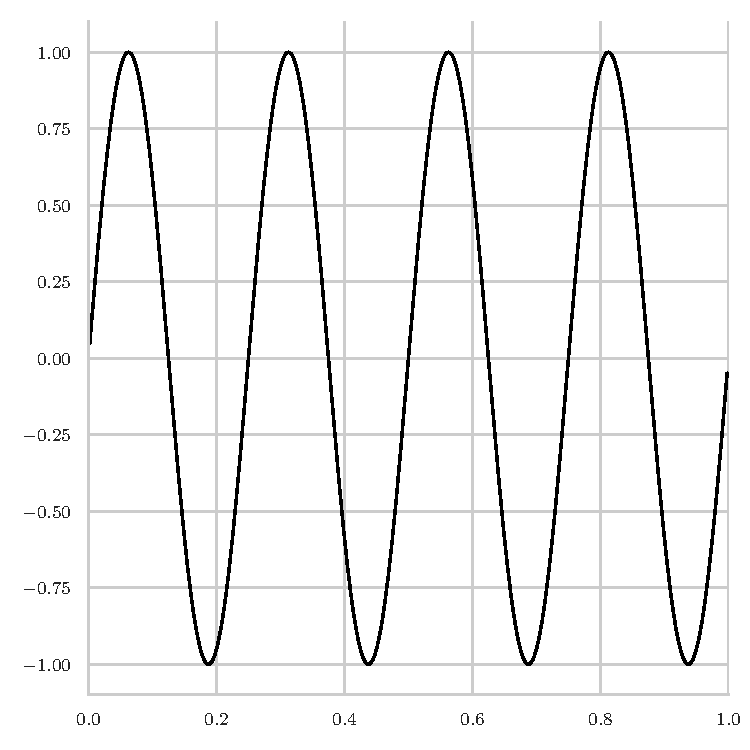
\includegraphics[width=\textwidth]{figures/initial_error_jacobi_8pi.pdf}
		%\caption{Initial Error}
	\end{subfigure}
	\hfill
	\begin{subfigure}[b]{0.45\textwidth}
		\centering
		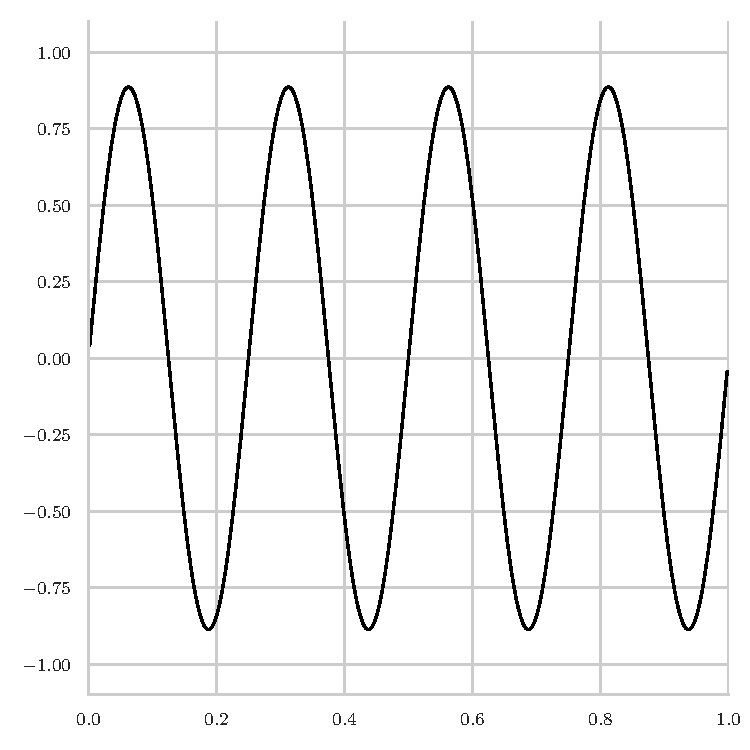
\includegraphics[width=\textwidth]{figures/final_error_jacobi_8pi.pdf}
		%\caption{Error after 100 Steps of weighted Jacobi}
	\end{subfigure}
	\begin{subfigure}[b]{0.45\textwidth}
		\centering
		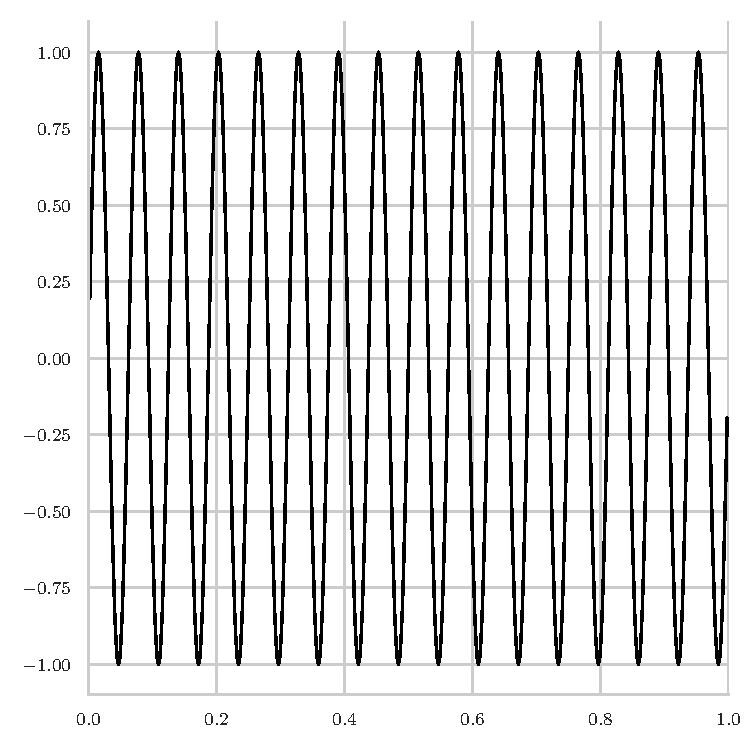
\includegraphics[width=\textwidth]{figures/initial_error_jacobi_32pi.pdf}
		%\caption{Initial Error}
	\end{subfigure}
	\hfill
	\begin{subfigure}[b]{0.45\textwidth}
		\centering
		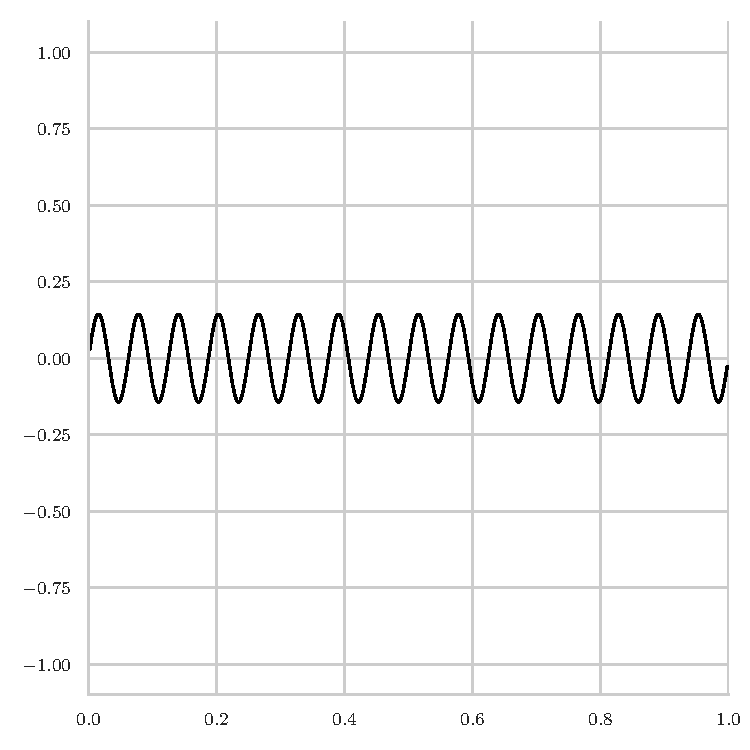
\includegraphics[width=\textwidth]{figures/final_error_jacobi_32pi.pdf}
		%\caption{Error after 100 Steps of weighted Jacobi}
	\end{subfigure}
	\begin{subfigure}[b]{0.45\textwidth}
		\centering
		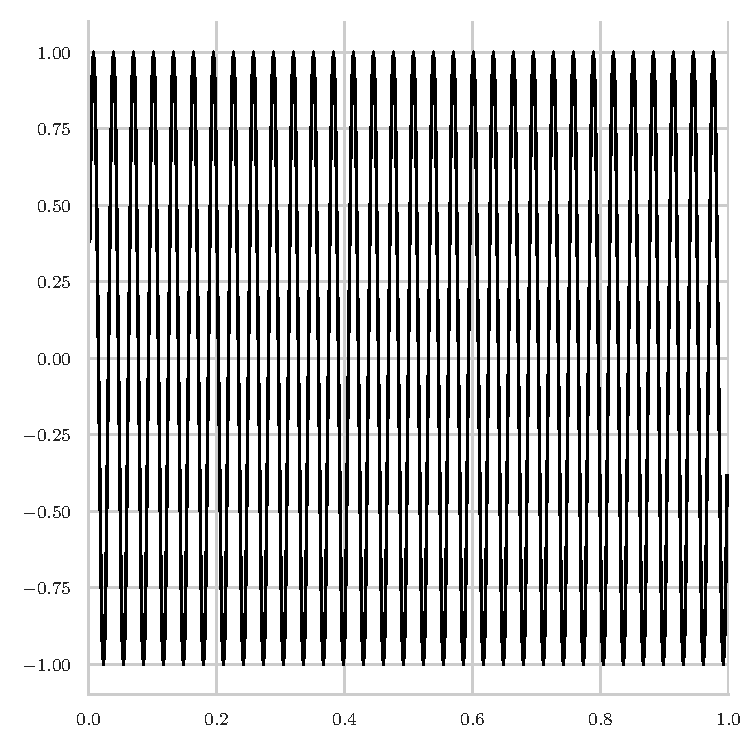
\includegraphics[width=\textwidth]{figures/initial_error_jacobi_64pi.pdf}
		%\caption{Initial Error}
	\end{subfigure}
	\hfill
	\begin{subfigure}[b]{0.45\textwidth}
		\centering
		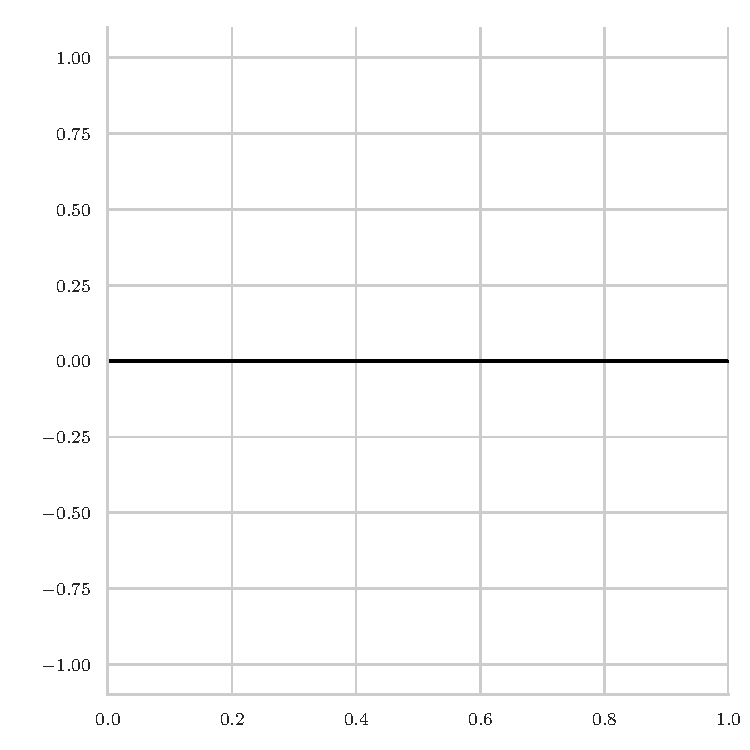
\includegraphics[width=\textwidth]{figures/final_error_jacobi_64pi.pdf}
		%\caption{Error after 100 Steps of weighted Jacobi}
	\end{subfigure}
	\caption{Different error components before and after 100 steps of Jacobi.}
	\label{fig:different-error-components-jacobi}
\end{figure}
Here, the left column shows the initial error while the right one includes the remaining one after applying 100 Jacobi steps.
Note that the frequency of change increases from top to bottom, whereas the amplitude of the error is always the same.
As it becomes apparent from investigating the right column of Figure~\ref{fig:different-error-components-jacobi}, the Jacobi method is not able to achieve a significant reduction of those error components with a low frequency of change within 100 iterations, which can be seen in the first example.
In contrast, the third example, which represents a highly-oscillating component, the error is already reduced to less than one-fifth of its original value throughout the domain.
By means of Figure~\ref{fig:different-error-components-gauss-seidel} the same behavior can also be observed for the Gauss-Seidel method, whereby, compared to the Jacobi method, high-frequency error components are reduced even faster.
\begin{figure}
	\centering
	\begin{subfigure}[b]{0.45\textwidth}
		\centering
		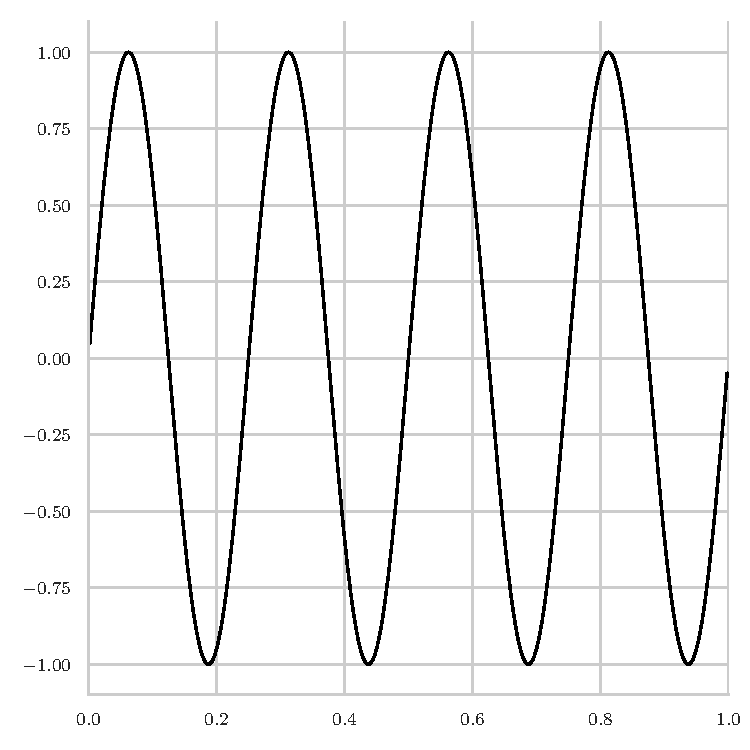
\includegraphics[width=\textwidth]{figures/initial_error_gauss_seidel_8pi.pdf}
		%\caption{Initial Error}
	\end{subfigure}
	\hfill
	\begin{subfigure}[b]{0.45\textwidth}
		\centering
		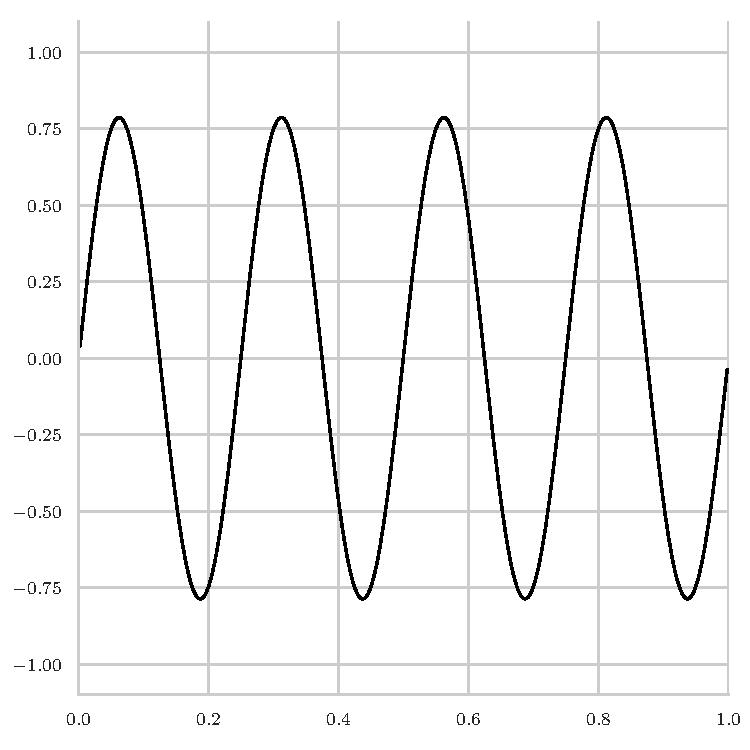
\includegraphics[width=\textwidth]{figures/final_error_gauss_seidel_8pi.pdf}
		%\caption{Error after 100 Steps of weighted Jacobi}
	\end{subfigure}
	\begin{subfigure}[b]{0.45\textwidth}
		\centering
		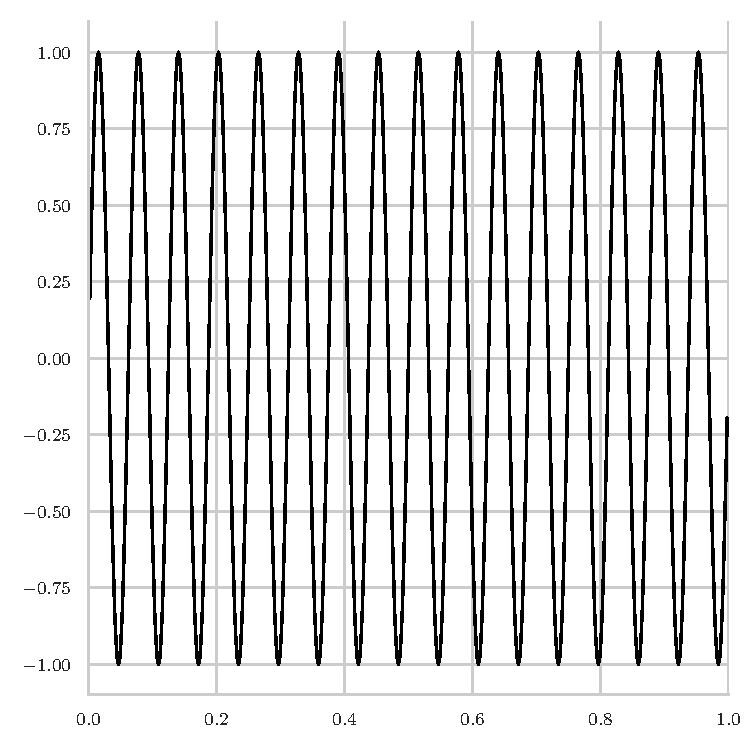
\includegraphics[width=\textwidth]{figures/initial_error_gauss_seidel_32pi.pdf}
		%\caption{Initial Error}
	\end{subfigure}
	\hfill
	\begin{subfigure}[b]{0.45\textwidth}
		\centering
		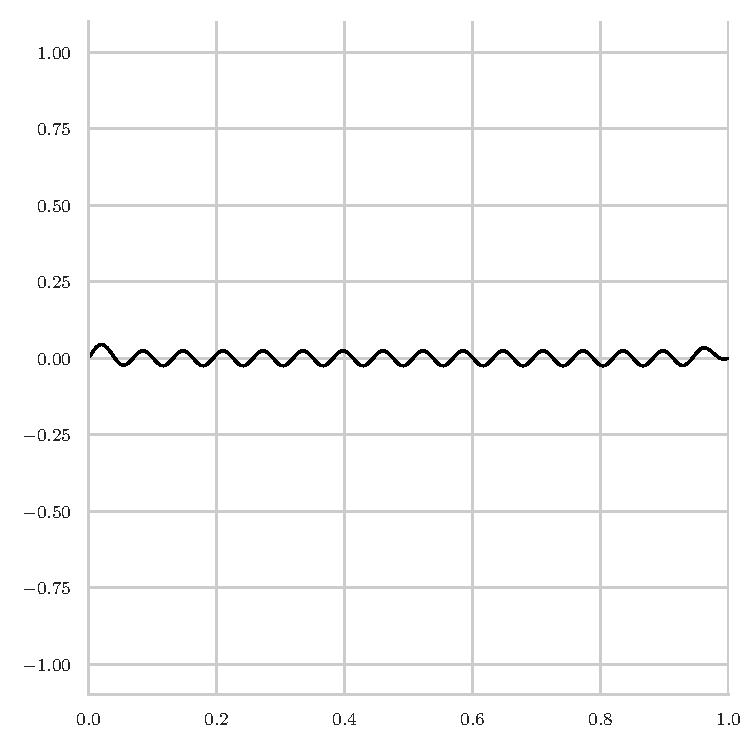
\includegraphics[width=\textwidth]{figures/final_error_gauss_seidel_32pi.pdf}
		%\caption{Error after 100 Steps of weighted Jacobi}
	\end{subfigure}
	\begin{subfigure}[b]{0.45\textwidth}
		\centering
		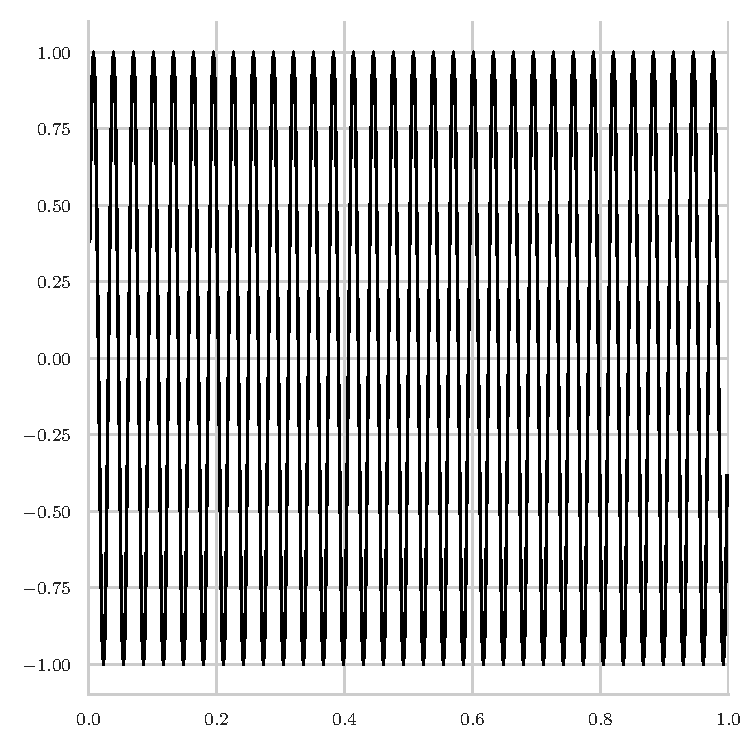
\includegraphics[width=\textwidth]{figures/initial_error_gauss_seidel_64pi.pdf}
		%\caption{Initial Error}
	\end{subfigure}
	\hfill
	\begin{subfigure}[b]{0.45\textwidth}
		\centering
		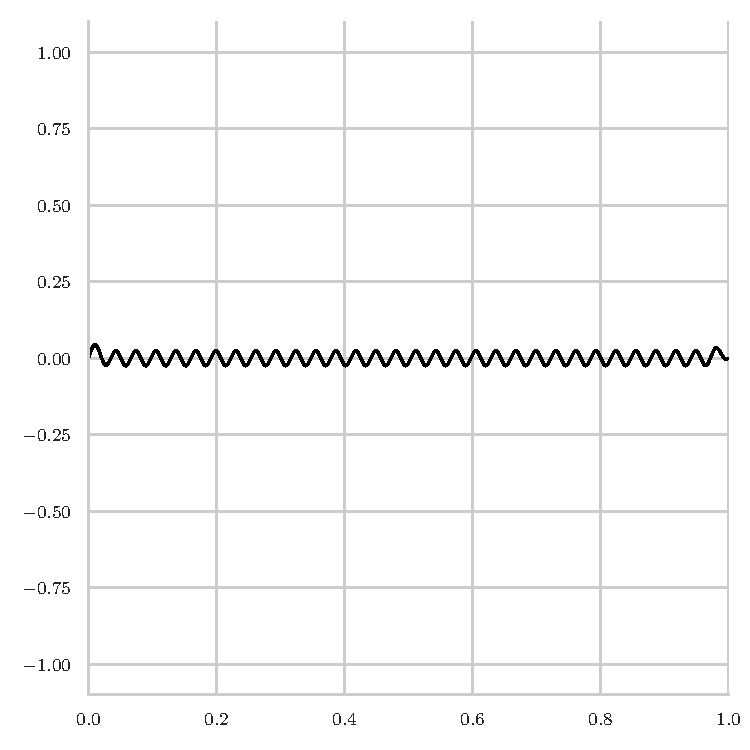
\includegraphics[width=\textwidth]{figures/final_error_gauss_seidel_64pi.pdf}
		%\caption{Error after 100 Steps of weighted Jacobi}
	\end{subfigure}
	\caption{Different error components before and after 100 steps of Gauss-Seidel.}
	\label{fig:different-error-components-gauss-seidel}
\end{figure}

We can further illustrate the error reduction properties of basic iterative methods by investigating Figure~\ref{fig:combined-error-jacobi} which shows the combination of two error components with equal magnitude, one of them with low, the other one with high frequency.
Again, the left plot shows the initial while the right one contains the reduced error after 100 iterations of Jacobi.
As it can be seen here, the attained improvement can be almost fully attributed to the reduction of the highly-oscillating component.
\begin{figure}
	\begin{subfigure}[b]{0.45\textwidth}
	\centering
		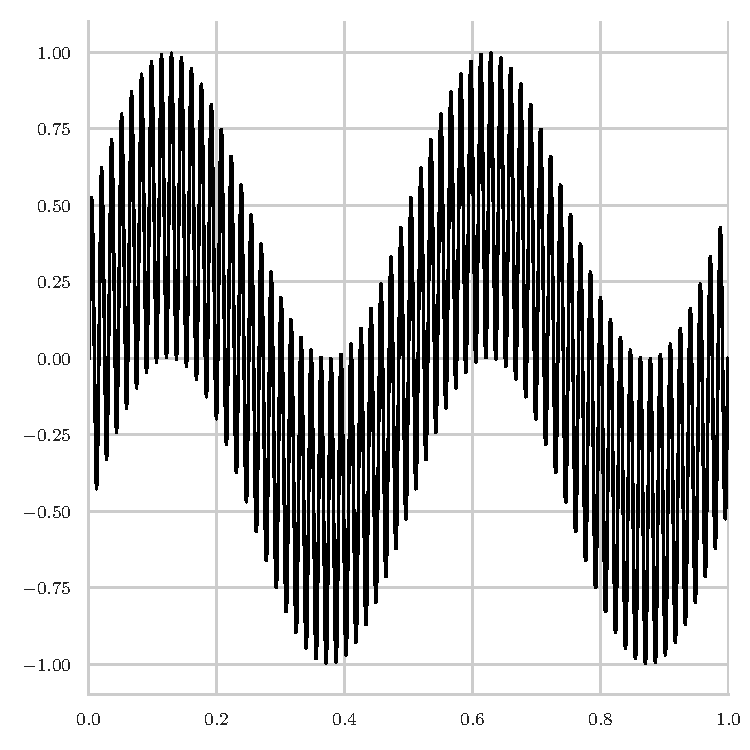
\includegraphics[width=\textwidth]{figures/initial_error_jacobi_combined.pdf}
\end{subfigure}
\hfill
\begin{subfigure}[b]{0.45\textwidth}
	\centering
		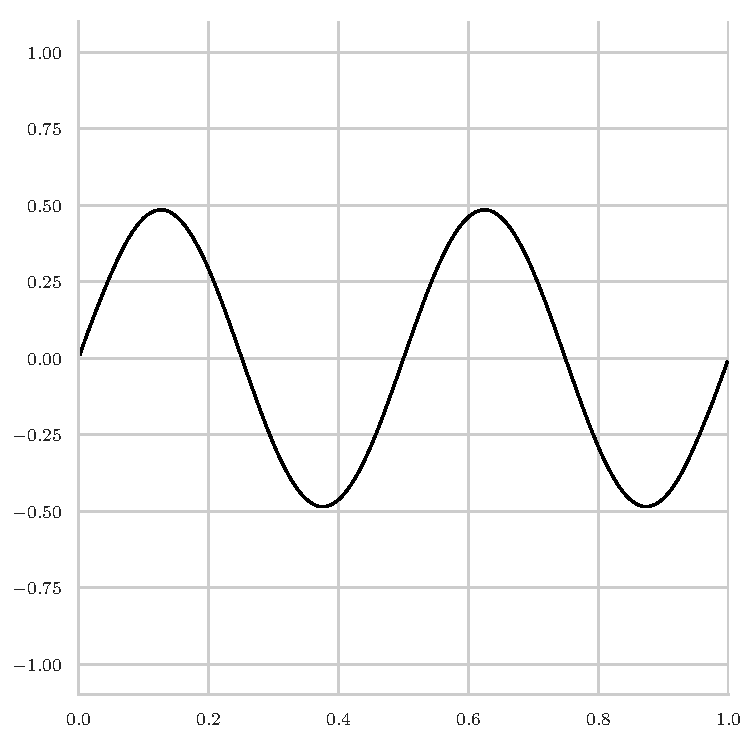
\includegraphics[width=\textwidth]{figures/final_error_jacobi_combined.pdf}
\end{subfigure}
	\caption{Combination of two error components before and after 100 steps of Jacobi.}
\label{fig:combined-error-jacobi}
\end{figure}
